\documentclass[final,hyperref={pdfpagelabels=false}]{beamer}
\usepackage{grffile}
\mode<presentation>{\usetheme{_bauer}}
\usepackage[english]{babel}
\usepackage[latin1]{inputenc}
\usepackage{amsmath, amsthm, amssymb, latexsym}
\usepackage{pifont} % for \ding symbols
\usepackage{multirow}
\usepackage{ragged2e} % for \justify
\let\olditem\item
\renewcommand\item{\justifying\olditem} % NOTE: This justify-alignes itemize-items, but heavily influences
% the rest of the document, s.t. the center-environment isn't working correctly anymore -> use \centering instead!

\usepackage{mdframed}
\newmdenv[%
  backgroundcolor=koalawhitegray4,
  linecolor=goodgreen,
  linewidth=3pt,
  topline=false,
  rightline=false,
  bottomline=false]{mdleftgreen}
\newmdenv[%
  backgroundcolor=koalawhitegray4,
  linecolor=badred,
  linewidth=3pt,
  topline=false,
  rightline=false,
  bottomline=false]{mdleftred}
\newmdenv[%
  backgroundcolor=koalawhitegray4,
  linecolor=koaladarkestblue,
  linewidth=3pt,
  topline=false,
  rightline=false,
  bottomline=false]{mdleftblue}
%\usepackage{times}\usefonttheme{professionalfonts}  % obsolete
%\usefonttheme[onlymath]{serif}
%\boldmath % macht ALLE Gleichungen automatisch fett
\usepackage[orientation=portrait,size=a0,scale=1.4,debug]{beamerposter}
% change list indention level
% \setdefaultleftmargin{3em}{}{}{}{}{}



% Eigene Befehle und Einstellungen -------------------------
\newcommand{\grayHeader}[1]{\textcolor{koaladarkgray}{{\large #1} \vspace{2ex}}}
\newcommand{\bfBlue}[1]{\textcolor{koaladarkestblue}{\textbf{#1}}}
\newcommand{\bfDarkgray}[1]{\textcolor{koaladarkgray}{\textbf{#1}}}
\newcommand{\blue}[1]{\textcolor{koaladarkestblue}{#1}}
\newcommand{\badred}[1]{\textcolor{badred}{#1}}
\newcommand{\goodgreen}[1]{\textcolor{goodgreen}{#1}}
\newcommand{\darkgray}[1]{\textcolor{koaladarkgray}{#1}}
\newcommand{\lightgray}[1]{\textcolor{koalagray}{#1}}
\newcommand{\fndarkgray}[1]{\textcolor{koaladarkgray}{\footnotesize #1}}
\newcommand{\fnlightgray}[1]{\textcolor{koalagray}{\footnotesize #1}}
\newcommand{\colHeader}[1]{
  \vspace{-3ex}
  \begin{center}\centering
  \bfBlue{#1}
  \end{center}
  \vspace{-2ex}
  \textcolor{koalablue}{\hrule{}}
  \vspace{2ex}
}
% Numbers with circles around it for headers
\usepackage{tikz}
\newcommand*\circled[1]{\tikz[baseline=(char.base)]{
\node[shape=circle,draw,inner sep=2pt] (char) {#1};}}
% Make figures get numbers (Figure 1, ...)
\setbeamertemplate{caption}[numbered]
% Change style of figure caption label
\usepackage[font={footnotesize,it,color=black}]{caption}
\captionsetup[figure]{labelfont={color=black}}
\captionsetup[figure]{labelfont=bf}
% Highlight text parts with a color block with rounded corners
\usepackage{tcolorbox}
\newtcbox{\mybox}{nobeforeafter,colframe=chocolate4,colback=verylightgray,boxrule=2pt,arc=4pt,
  boxsep=0pt,left=6pt,right=6pt,top=6pt,bottom=6pt,tcbox raise base}
% Eigene Befehle Ende --------------------------------------



%\usepackage{snapshot} % will write a .dep file with all dependencies, allows for easy bundling

\usepackage{array,booktabs,tabularx}
\newcolumntype{Z}{>{\centering\arraybackslash}X} % centered tabularx columns
\newcommand{\pphantom}{\textcolor{ta3aluminium}} % phantom introduces a vertical space in p formatted table columns??!!

  \listfiles

%%%%%%%%%%%%%%%%%%%%%%%%%%%%%%%%%%%%%%%%%%%%%%%%%%%%%%%%%%%%%%%%%%%%%%%%%%%%%%%%%%%%%%
\graphicspath{{figures/}}

\title{\huge{KOALA: Estimating coalition probabilities}\\[0.5ex]\LARGE{in multi-party electoral systems}}
\author{Alexander Bauer$^{1}$, Andreas Bender$^{1}$, Andr\'e Klima$^{1}$, Helmut K\"{u}chenhoff$^{1}$}
\institute[LMU Munich]{\textit{$^{1}$ Statistical Consulting Unit StaBLab, Department of Statistics, LMU Munich,
Germany} \\[2ex] \texttt{Alexander.Bauer@stat.uni-muenchen.de}}
\date[July 18th, 2018]{July 18th, 2018}

%%%%%%%%%%%%%%%%%%%%%%%%%%%%%%%%%%%%%%%%%%%%%%%%%%%%%%%%%%%%%%%%%%%%%%%%%%%%%%%%%%%%%%
  \newlength{\columnheight}
\setlength{\columnheight}{105cm}


%%%%%%%%%%%%%%%%%%%%%%%%%%%%%%%%%%%%%%%%%%%%%%%%%%%%%%%%%%%%%%%%%%%%%%%%%%%%%%%%%%%%%%

% Begin page ----------------------------------------------
\begin{document}
\begin{frame}
\begin{columns}
\begin{column}{1\textwidth} % 1 Seite, die die ganze Seite einnimmt


% Motivation ---------------------------------------------
\begin{beamercolorbox}[center,wd=\textwidth]{postercolumn}
\begin{minipage}[T]{.95\textwidth}  % tweaks the width, makes a new \textwidth
\begin{block}{\footnotesize Motivation}
  \begin{center}\centering
  \grayHeader{Election poll-based reporting}
  \end{center}

  % Upper columns with general description -----
  \begin{columns}[t]

  \begin{column}{.475\textwidth}
  \colHeader{What's the status quo?}
  Typical election poll reporting: \\[1cm]
  \begin{tabular}{p{9cm}p{25cm}}
  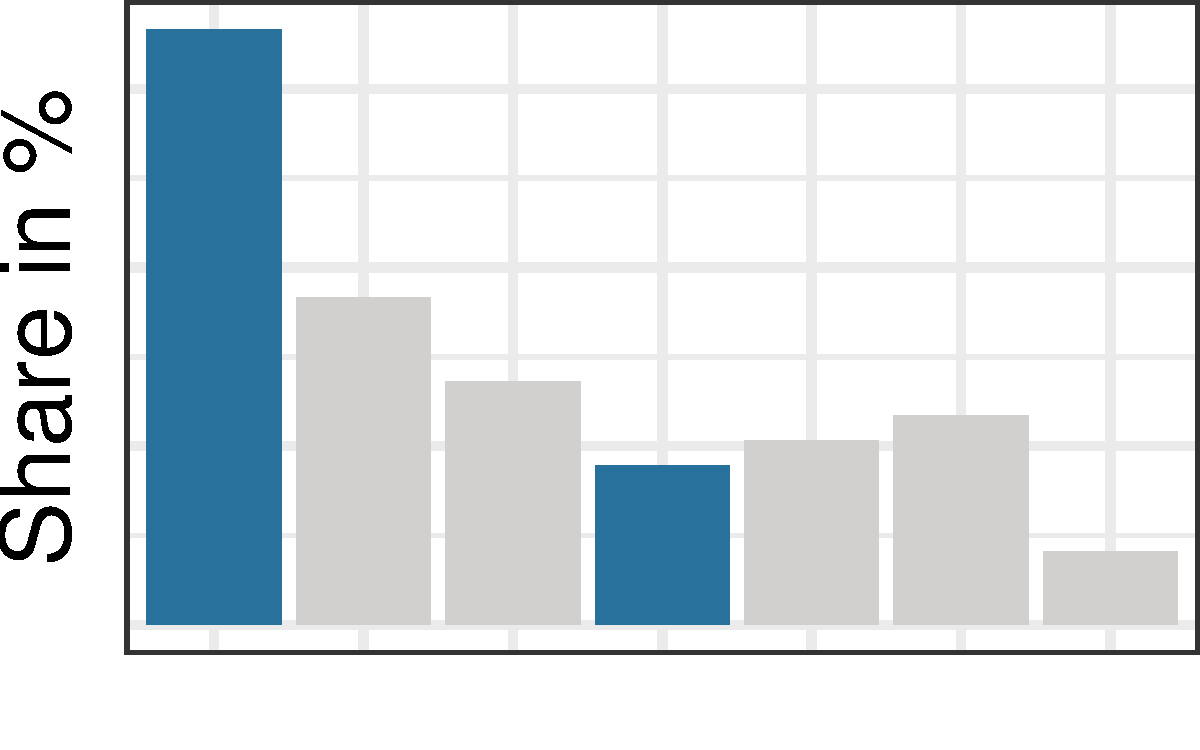
\includegraphics[height=5.75cm]{figures/motivation_survey_highlighted}
  &
  \vspace{-5.3cm}
  \begin{itemize}
    \item is based on observed mean voter shares
    \item sets the focus on individual party achievements
    \item imparts sample uncertainty only insufficiently
  \end{itemize}
  \end{tabular}
  \\[10px]
  \begin{mdleftblue}
  \begin{minipage}{\textwidth}
  \lightgray{\footnotesize Typical headline:}
  \\
  \vspace{-50px}
  \textit{\darkgray{``The two parties jointly obtain} \blue{48\% of all votes}\darkgray{.''}}
  \\[17px]
  \end{minipage}
  \end{mdleftblue}
  \vspace{50px}
  % Example header
  {
  \setlength{\fboxrule}{3pt} % Border thickness
  \fcolorbox{koalawhitegray}{koalawhitegray2}{
  \begin{minipage}{0.9\textwidth}
  \vspace{2.5ex}
  \begin{center}\centering
  \bfBlue{Real-world Example} \\
  {\footnotesize \lightgray{Reporting on}} \darkgray{Union} {\footnotesize \lightgray{and}} \darkgray{FDP} {\footnotesize \lightgray{to jointly obtain a majority before the German federal election 2013}}
  \end{center}
  \vspace{2ex}
  \end{minipage}
  }
  }
  \end{column}

  % \hspace{-3.1ex}
  % \textcolor{LMUlightgray}{\vrule{}}
  % \hspace{3.1ex}

  \begin{column}{.475\textwidth}
  \colHeader{What do we propose?}
  Proposed type of reporting: \\[1cm]
  \begin{tabular}{p{9cm}p{25cm}}
  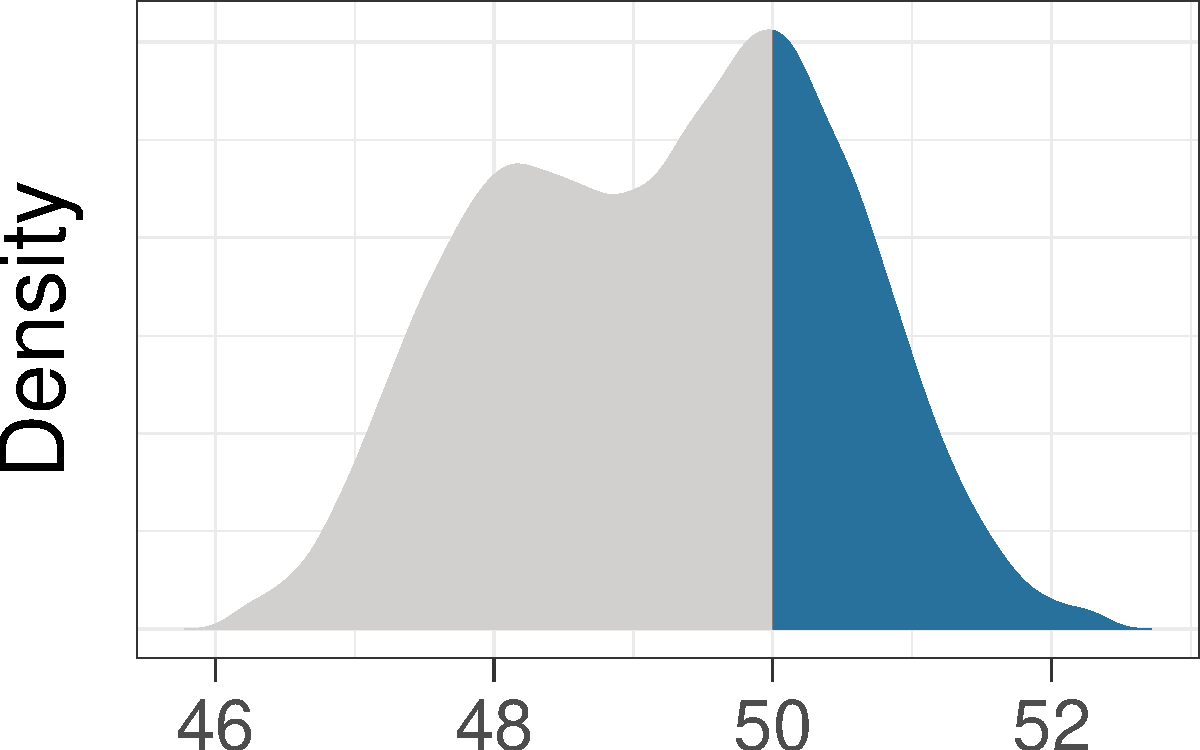
\includegraphics[height=5.75cm]{figures/motivation_density_highlighted}
  &
  \vspace{-5.3cm}
  \begin{itemize}
    \item focuses on specific events (e.g. potential majorities)
    \item naturally imparts sample uncertainty using probabilities
    \item prevents misunderstandings by using this holistic approach
  \end{itemize}
  \end{tabular}
  \\[10px]
  \begin{mdleftblue}
  \begin{minipage}{\textwidth}
  \lightgray{\footnotesize Proposed headline:}
  \\
  \vspace{-50px}
  \textit{\darkgray{``The two parties have a} \blue{probability of 32\%} \darkgray{to jointly obtain a majority.''}}
  \\[17px]
  \end{minipage}
  \end{mdleftblue}
  \vspace{60px}

  We aim to \textbf{shift the focus} from \\[1.3ex]
  \begin{tabular}{clccl}
  \multirow{2}{*}[-0.95ex]{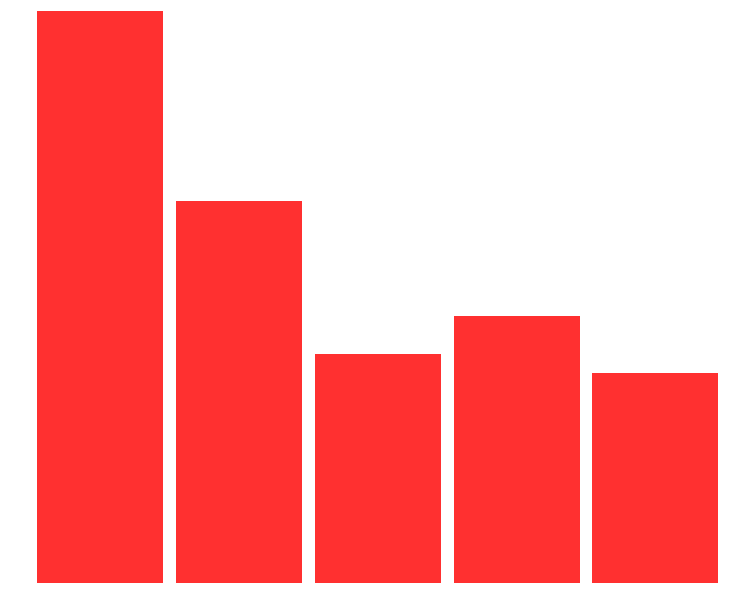
\includegraphics[height=3ex]{figures/motivation_pictoBar_col}} &
  \darkgray{\footnotesize Incomprehensive} &
  \multirow{2}{*}{\ \ \darkgray{to} \ } &
  \multirow{2}{*}[-1ex]{
\includegraphics[height=3ex]{figures/motivation_pictoDens_col}} &
  \darkgray{\footnotesize Uncertainty-based} \\
   & observed party shares & & & event probabilities \\
  \end{tabular}
  \end{column}

  \end{columns}

  % \noindent\hfil\textcolor{LMUlightgray}{\rule{0.93\textwidth}{.4pt}}\hfil
  % % \textcolor{LMUlightgray}{\hrule{}}
  % \vspace{3ex}

  % Lower columns with a specific example ----
  {
  \vspace{-4pt}
  \hspace{-24.34pt}
  \setlength{\fboxrule}{3pt} % Border thickness
  \fcolorbox{koalawhitegray}{koalawhitegray3}{
  \begin{minipage}{.96\textwidth}
  \vspace{3ex}
  \begin{columns}[t]

  \begin{column}{.29\textwidth}
  \darkgray{Last pre-election opinion poll:} \lightgray{\tiny Source: Forsa, 20.09.2013}
  \\[2.5ex]
  \begin{center}\centering
  % \scalebox{0.75} & {\footnotesize \lightgray{26\%}} & {\footnotesize \lightgray{10\%}} & \darkgray{5\%} & {\footnotesize \lightgray{9\%}} & {\footnotesize \lightgray{4\%}} & {\footnotesize \lightgray{6\%}} \\
  \bottomrule
  \end{tabular}
  % }
  \end{center}
  \vspace{1.5ex}
  \begin{center}\centering
  \darkgray{After redistribution} \lightgray{\footnotesize of party votes $<$5\% \\ (i.e. the minimum vote share to enter the German parliament)} \\
  \darkgray{Union-FDP} \lightgray{\footnotesize jointly} \darkgray{obtain} \lightgray{\footnotesize exactly} \darkgray{50\%}.
  \end{center}
  \vspace{-3ex}
  \textcolor{koalablue}{$$ \underbrace{\resizebox{\hsize}{!}{ }}_{ } $$}
  \ \\ \vspace{-2ex}
  \begin{mdleftred}
  \begin{minipage}{\textwidth}
  \lightgray{\footnotesize Media headline:}
  \\
  \begin{center}\centering
  \vspace{-2ex}
  \darkgray{\textit{``Union-FDP loses its majority''}}
  \vspace{-.2ex}
  \end{center}
  \lightgray{\tiny Source: FAZ.net (2017). Umfrage zur Bundestagswahl: Schwarz-Gelb verliert \\[-2ex]
  die Mehrheit.http://archive.is/SuXVt. Accessed 26 April 2018.}
  \end{minipage}
  \end{mdleftred}
  \end{column}

  \begin{column}{.025\textwidth}
  \vspace{11ex}
  \huge{\blue{\ding{223}}}
  \end{column}

  \begin{column}{.26\textwidth}
  Flaws of this type of reporting:
  \vspace{1.5ex}
  \begin{itemize}
    \item \darkgray{Misleading conclusions are drawn} \\[0.2cm] \fnlightgray{A mean share of 50\% only means that it's} \fndarkgray{slightly more probable} \fnlightgray{to miss a majority}
    \item \darkgray{Sample uncertainty is ignored} \\[0.2cm] \fnlightgray{E.g., with a mean voter share of 5\%, FDP will only enter the parliament with $\approx$50\%}
    \item \darkgray{Redistribution of votes is ignored} \\[0.2cm] \fnlightgray{FAZ.net bases the conclusion on the observed voter share and not on the redistributed 50\% share}
  \end{itemize}
  \end{column}

  \begin{column}{.025\textwidth}
  \vspace{11ex}
  \huge{\blue{\ding{223}}}
  \end{column}

  \begin{column}{.29\textwidth}
  Foundations of KOALA-based reporting:
  \vspace{1.5ex}
  \begin{itemize}
    \item \darkgray{Use event \textbf{probabilities}} \fnlightgray{instead of voter shares} \\[0.2cm] \fnlightgray{Probabilities comprise sample uncertainty in a natural way and are less at risk to be misinterpreted}
    \item \darkgray{Use \textbf{event} probabilities} \fnlightgray{instead of voter shares} \\[0.2cm] \fnlightgray{Focusing on the main events allows the reader to easily grasp the big picture}
  \end{itemize}
  \vspace{-1.7ex}
  \textcolor{koalablue}{$$ \underbrace{\resizebox{\hsize}{!}{ }}_{ } $$}
  \ \\ \vspace{-2ex}

  \begin{mdleftgreen}
  \begin{minipage}{\textwidth}
  \lightgray{\footnotesize KOALA headline:}
  \begin{center}\centering
  \darkgray{\textit{
  ``Union-FDP gains seat majority with 26\%, \ \ \\[0.1cm] \ \ FDP passes into parliament with 51\%$^*$''
  }}
  \end{center}
  \vspace{-0.7ex}
  \lightgray{\tiny ${}^*$ If the election was held today}
  \end{minipage}
  % }
  \end{mdleftgreen}
  \end{column}
  \end{columns}
  \end{minipage}
  }
  }

  \vspace{1ex}
\end{block}
\end{minipage}
\end{beamercolorbox}



% Begin main part -----------------------------------
\vspace{2ex}
\begin{columns}[T]

% empty space on left
\begin{column}{.016\textwidth}
\end{column}

\begin{column}{.484\textwidth}
\begin{beamercolorbox}[center,wd=\textwidth]{postercolumn}
\begin{minipage}[T]{.95\textwidth}  % tweaks the width, makes a new \textwidth
% \parbox[t][\columnheight]{\textwidth}{ % must be some better way to set the the height, width and textwidth simultaneously
% Since all columns are the same length, it is all nice and tidy.  You have to get the height empirically


% Methodology ---------------------------------------
\begin{block}{\footnotesize Event probability estimation}
\bfBlue{Estimating event probabilities}
% \\[0.5cm]
\\[0.05cm]
\textcolor{LMUlightgray}{\hrule{}}
\vspace{1ex}
\hspace*{-40px}
\begin{minipage}{\textwidth}
\begin{columns}[t]
  \begin{column}{.01\textwidth}
  \vspace{7px}
  \begin{minipage}{\textwidth}
  \bfBlue{1} \\
  \vspace{46px}
  \bfBlue{2} \\
  \vspace{14px}
  \bfBlue{3}
  \end{minipage}
  \end{column}

  \hspace{-30px}
  \textcolor{LMUlightgray}{\vrule{}}
  \hspace{0px}

  \begin{column}{.93\textwidth}
  \vspace{7px}
  \begin{minipage}{\textwidth}
  \darkgray{\textbf{Multinomial-Dirichlet model}}
%with uninformative prior
for the true party shares $\theta_j$ {\footnotesize (Gelman et al., 2013)}:
$$
(\theta_1,\ldots,\theta_k)^T \sim Dirichlet(\alpha_1,\ldots,\alpha_k), \ \ \text{with} \ \ \alpha_1 = \ldots = \alpha_k = \frac{1}{2}
$$
% $$
% \begin{aligned}
% \boldmath{\theta} &= (\theta_1,\ldots,\theta_k)^\T \sim Dirichlet(\alpha_1,\ldots,\alpha_k), \\
% \text{with} &\ \ \ \ \ \ \ \ \ \ \ \ \ \ \ \alpha_1 = \ldots = \alpha_k = \frac{1}{2}
% \end{aligned}
% $$
Given one survey, we obtain a \darkgray{\textbf{Dirichlet posterior}}
with $\alpha_j = x_j + \frac{1}{2}$ for each party $j=1,\ldots,k$ and its observed
vote counts $x_j$.
\\[0.5cm]
Using \darkgray{\textbf{Monte Carlo simulations}} of election outcomes, we obtain
obtain specific event probabilities by calculating the relative frequency of their
occurrence.
% As vote shares are usually rounded before publication,
% we adjust the available data by adding random noise to $x_j$ before
% calculating the Bayesian posterior.
% we add uniformly distributed random noise $r_\gamma \sim U[-\gamma,\gamma]$ to the shares (e.g., $\gamma = 0.5\%$) and rescale the sum to $100\%$.
  \end{minipage}
  \vspace{7px}
  \end{column}
\end{columns}
\end{minipage}

\vspace{1ex}
\textcolor{LMUlightgray}{\hrule{}}
\vspace{5ex}

% In the presence of multiple published opinion polls, pooling is used to summarize the observed results in order to reduce sample uncertainty. To assure a reliable pooling regarding the current public opinion, we only use polls published within the past 14 days and only use the most recent survey published by each polling agency.
\bfBlue{Pooling multiple surveys} \\[0.5cm]
We pool the most recent surveys within the past 14 days (one per polling agency) to reduce
sample uncertainty. We adjust the uncertainty of the \darkgray{multinomially distributed}
summed number of votes per party by using an \darkgray{\textbf{effective sample size}} {\footnotesize (Hanley et al., 2003)}.
% \\[0.5cm]
\\[0.05cm]
\textcolor{LMUlightgray}{\hrule{}}
\vspace{1ex}
\hspace*{-40px}
\begin{minipage}{\textwidth}
\begin{columns}[t]
  \begin{column}{.01\textwidth}
  \vspace{7px}
  \begin{minipage}{\textwidth}
  \bfBlue{1} \\
  \vspace{284px}
  \bfBlue{2}
  \end{minipage}
  \end{column}

  \hspace{-30px}
  \textcolor{LMUlightgray}{\vrule{}}
  \hspace{0px}

  \begin{column}{.93\textwidth}
  \vspace{7px}
  \begin{minipage}{\textwidth}
As polls from different polling agencies are correlated, \darkgray{\textbf{party-specific correlations}} were
estimated based on 20 surveys of polling agencies Emnid and Forsa, using
$$
Cov(X_{Aj}, X_{Bj}) = \frac{1}{2} \cdot \left(Var(X_{Aj}) + Var(X_{Bj}) - Var(X_{Aj} - X_{Bj}) \right),
$$
\darkgray{\footnotesize with \\}
\begin{minipage}{\textwidth}
\hspace{0.5in}
\begin{itemize}
  \item \darkgray{\footnotesize $X_{Sj}$ the observed votes for party $j$ in survey $S$,}
  \item \darkgray{\footnotesize $Var(X_{Aj})$, $Var(X_{Bj})$ the theoretical variances of binomial distributions,}
  \item \darkgray{\footnotesize $Var(X_{Aj} - X_{Bj})$ estimated from the party share differences.}
\end{itemize}
\end{minipage}
\\[0.8cm]
For simplicity, we set the correlation to a fixed value of $0.5$.
\\[0.5cm]
The \darkgray{\textbf{effective sample size}} $n_{\text{eff}}$ is then defined as the ratio between
the estimated variance for the pooled sample and the theoretical variance for a
sample of size one: \\[0.1cm]
$$
n_{\text{eff}} = \frac{Var(\text{pooled})}{Var(\text{sample of size one})}
$$
  \end{minipage}
  \vspace{7px}
  \end{column}
\end{columns}
\end{minipage}
\vspace{1ex}
\textcolor{LMUlightgray}{\hrule{}}

% Quantification of pairwise correlation is done based on the variance of the
% difference between two polls. The following equation holds for two independent
% random sample polls $A$ and $B$:
%
% $$
% \begin{aligned}
% %Var(X_A - X_B) &= Var(X_A) + Var(X_B) - 2 \cdot Cov(X_A, X_B) \\
% Cov(X_{Aj}, X_{Bj}) &= \frac{1}{2} \cdot \left(Var(X_{Aj}) + Var(X_{Bj}) - Var(X_{Aj} - X_{Bj}) \right).
% \end{aligned}
% $$
%
% We take $Var(X_{Aj})$ and $Var(X_{Bj})$ as the theoretical variances of the binomially distributed, observed voter numbers and estimate $Var(X_{Aj} - X_{Bj})$ based on the observed differences between the party shares. Having done so, one can estimate the covariance $Cov(X_{Aj}, X_{Bj})$ and accordingly also the correlation. As the binomial distribution is directly proportional to the sample size, the effective sample size $n_{\text{eff}}$ can be defined as the ratio between the estimated variance for the pooled sample and the theoretical variance of a sample of size one:
% $$
% n_{\text{eff}} = \frac{Var(\text{pooled})}{Var(\text{sample of size 1})},
% $$
% with, in the case of two surveys,
% $$
% Var(\text{pooled}) = Var(X_A + X_B) = Var(X_A) + Var(X_B) + 2 Cov(X_A,X_B)
% $$
% and $Var(\text{sample of size 1})$ the theoretical variance of the pooled share.
%
% Looking at the party-specific correlations between 20 surveys conducted by the two most regular German polling agencies, Emnid and Forsa, we on average end up with a medium high correlation, using mean party shares and sample sizes per institute for the theoretical variances. Other institute comparisons were not performed as too few surveys were conducted over comparable time frames. For simplicity, we set the correlation used in our methodology to $0.5$. For calculating $n_{\text{eff}}$ we base the calculation on the result of the biggest party, as the specific party choice only marginally affects $n_{\text{eff}}$.
\end{block}



% Begin second column of main part -----------------
\end{minipage}
\end{beamercolorbox}
\end{column}

\begin{column}{.484\textwidth}
\begin{beamercolorbox}[center,wd=\textwidth]{postercolumn}
\begin{minipage}[T]{.95\textwidth}  % tweaks the width, makes a new \textwidth


% Visualization ------------------------------------
\begin{block}{\footnotesize Visualization \& Implementation}
\bfBlue{Selected visualizations}
\\[0.05cm]
\textcolor{LMUlightgray}{\hrule{}}
\vspace{1ex}
\begin{columns}[t]
  \begin{column}{.3\textwidth}
  \begin{center}\centering
  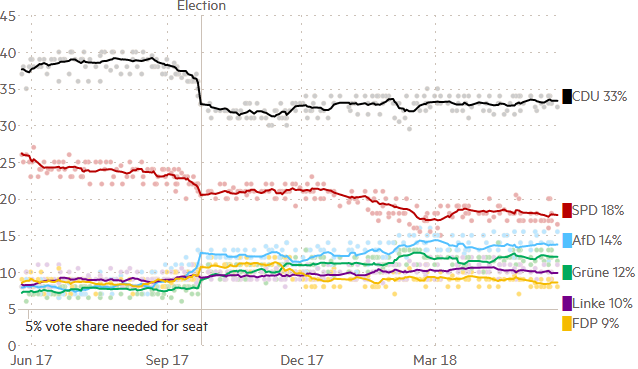
\includegraphics[height=120px]{figures/pooled_shares}
  \end{center}
  \end{column}

  \hspace{-1.5ex}
  \textcolor{LMUlightgray}{\vrule{}}
  \hspace{1.5ex}

  \begin{column}{.65\textwidth}
  \ \\
  \textbf{Adjusted line plots} are used to visualize the pooled voter shares are visualized, showing both the mean share and the corresponding uncertainty
  \end{column}
\end{columns}
\vspace{1ex}
\textcolor{LMUlightgray}{\hrule{}}
\vspace{1ex}
\begin{columns}[t]
  \begin{column}{.3\textwidth}
  \begin{center}\centering
  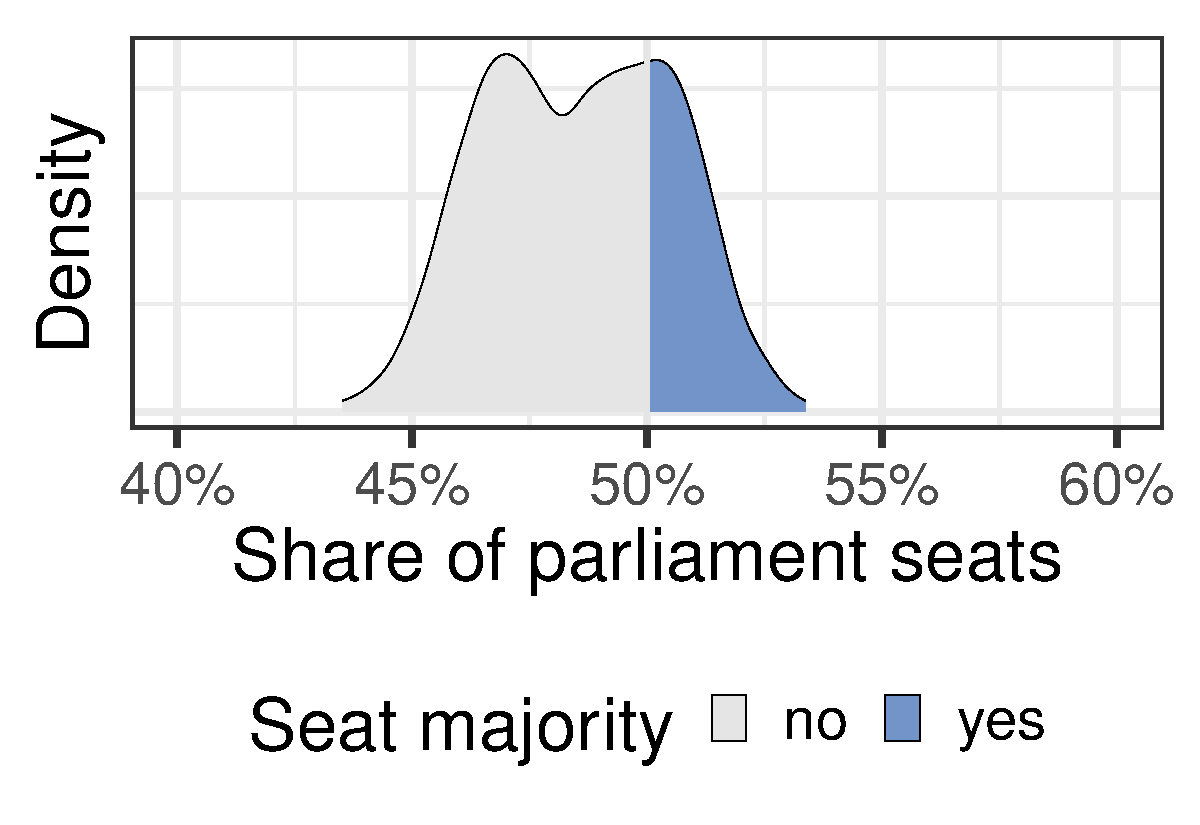
\includegraphics[height=120px]{figures/vis_seatDist}
  \end{center}
  \end{column}

  \hspace{-1.5ex}
  \textcolor{LMUlightgray}{\vrule{}}
  \hspace{1.5ex}

  \begin{column}{.65\textwidth}
  \ \\
  \textbf{Density plots} are used to depict one simulated seat distribution
  \end{column}
\end{columns}
\vspace{1ex}
\textcolor{LMUlightgray}{\hrule{}}
\vspace{1ex}
\begin{columns}[t]
  \begin{column}{.3\textwidth}
  \begin{center}\centering
  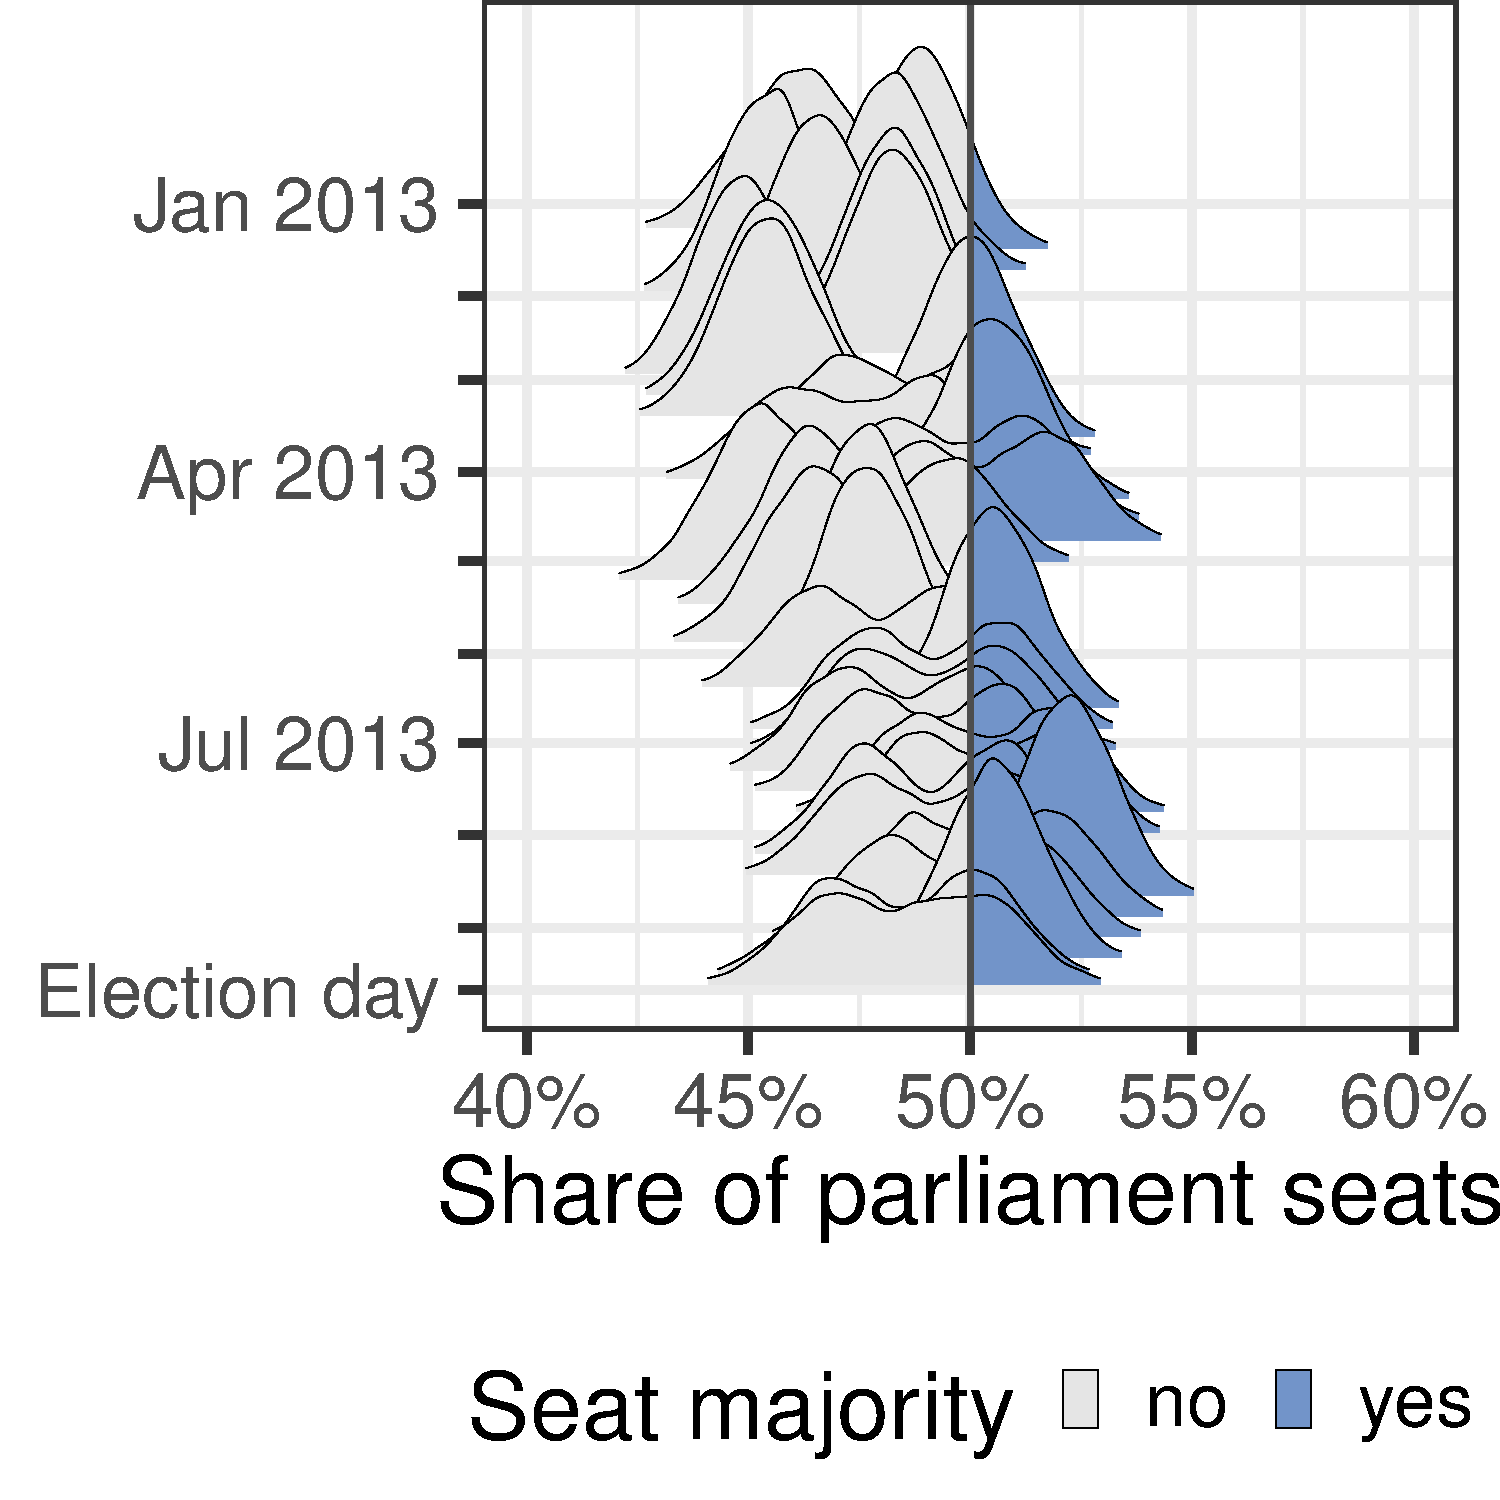
\includegraphics[height=250px]{figures/vis_seatDist_time}
  \end{center}
  \end{column}

  \hspace{-1.5ex}
  \textcolor{LMUlightgray}{\vrule{}}
  \hspace{1.5ex}

  \begin{column}{.65\textwidth}
  \ \\
  \textbf{Ridgeline plots} {\footnotesize (Wilke, 2017)} are used to depict the simulated seat distribution development over time
  \end{column}
\end{columns}
\vspace{1ex}
\textcolor{LMUlightgray}{\hrule{}}
\vspace{6ex}
\bfBlue{Implementation}
\\[0.05cm]
\textcolor{LMUlightgray}{\hrule{}}
\vspace{1ex}
% \vspace{-3ex}
\begin{columns}[t]
  \begin{column}{.45\textwidth}
  \begin{center}\centering
  
\includegraphics[height=3.5ex]{figures/Koala_Logo_ohneSchrift} \\
  \blue{\footnotesize \href{http://koala.stat.uni-muenchen.de}{koala.stat.uni-muenchen.de}}
  \end{center}
  \end{column}

  \hspace{-1.5ex}
  \textcolor{LMUlightgray}{\vrule{}}
  \hspace{1.5ex}

  \begin{column}{.45\textwidth}
  \begin{center}\centering
  
\includegraphics[height=3.5ex]{figures/implementation_twitter} \\
  \blue{\footnotesize \href{https://twitter.com/KOALA_LMU}{@KOALA\_LMU}}
  \end{center}
  \end{column}
\end{columns}
\vspace{1ex}
\textcolor{LMUlightgray}{\hrule{}}
\vspace{3ex}

\darkgray{\textbf{Major building blocks}}
\begin{minipage}{\textwidth}
\hspace{0.5in}
\begin{itemize}
  \item The accompanying R package \bfBlue{\href{https://adibender.github.io/coalitions/}{\texttt{coalitions}}}
  \item An automated fetch-and-update process for the website
  \item An automated bot tweeting new results
\end{itemize}
\end{minipage}

% \bfBlue{Future goals} \\
% Making the approach known to reporters,
% our long-term goal is to make proper uncertainty assessment in general opinion
% poll-based reporting the rule, rather than an exception.

% % Footer with software icons
% \vspace{1ex}
% \textcolor{LMUlightgray}{\hrule{}}
% \vspace{1ex}
% \begin{columns}[t]
%   % \begin{column}{.1\textwidth}
%   % \begin{center}\centering
%   % 
\includegraphics[height=5ex]{figures/qr}
%   % \end{center}
%   % \end{column}
%   %
%   % \hspace{-1.5ex}
%   % \textcolor{LMUlightgray}{\vrule{}}
%   % \hspace{1.5ex}
%
%   \begin{column}{.15\textwidth}
%   \begin{center}\centering
%   \vspace{3ex}
%   
\includegraphics[height=4ex]{figures/implementation_r}
%   \end{center}
%   \end{column}
%
%   \hspace{-1.5ex}
%   \textcolor{LMUlightgray}{\vrule{}}
%   \hspace{1.5ex}
%
%   \begin{column}{.15\textwidth}
%   \begin{center}\centering
%   \vspace{3.8ex}
%   
\includegraphics[height=2.6ex]{figures/implementation_shiny}
%   \end{center}
%   \end{column}
%
%   \hspace{-1.5ex}
%   \textcolor{LMUlightgray}{\vrule{}}
%   \hspace{1.5ex}
%
%   \begin{column}{.15\textwidth}
%   \begin{center}\centering
%   
\includegraphics[height=8ex]{figures/qr}
%   \end{center}
%   \end{column}
%
%   \hspace{-1.5ex}
%   \textcolor{LMUlightgray}{\vrule{}}
%   \hspace{1.5ex}
%
%   \begin{column}{.15\textwidth}
%   \begin{center}\centering
%   \vspace{3ex}
%   
\includegraphics[height=4ex]{figures/implementation_sheets}
%   \end{center}
%   \end{column}
%
%   \hspace{-1.5ex}
%   \textcolor{LMUlightgray}{\vrule{}}
%   \hspace{1.5ex}
%
%   \begin{column}{.15\textwidth}
%   \begin{center}\centering
%   \vspace{3ex}
%   
\includegraphics[height=4ex]{figures/implementation_twitter}
%   \end{center}
%   \end{column}
% \end{columns}
\end{block}


% End main part ------------------------------------
\end{minipage}
\end{beamercolorbox}
\end{column}

% empty space on right
\begin{column}{.016\textwidth}
\end{column}

\end{columns}


% Literature ---------------------------------------
\vspace{2ex}
\begin{beamercolorbox}[center,wd=\textwidth]{postercolumn}
\begin{minipage}[T]{.95\textwidth}  % tweaks the width, makes a new \textwidth
\begin{block}{\footnotesize References}
{\footnotesize
Bender, A. and Bauer, A. (2018). coalitions: Coalition probabilities in multi-party democracies.
\textit{Journal of Open Source Software}, \textbf{3(23)}, 606,
\href{https://doi.org/10.21105/joss.00606}{\texttt{https://doi.org/10.21105/joss.00606}}. \\
Unser AStA-Paper no ois Technical Report? \\
Gelman, A. et al. (2013). \textit{Bayesian Data Analysis, 3rd edition}. Boca Raton, FL: CRC press. \\
Hanley, J. A. et al. (2003). Statistical analysis of correlated data using gen-
eralized estimating equations: an orientation. \textit{American journal of epidemiology},
\textbf{157(4)}, 364--375. \\
Wilke C.O. (2017). \textit{ggridges: Ridgeline Plots in 'ggplot2'}. R package version
0.4.1. URL \href{https://CRAN.R-project.org/package=ggridges}{https://CRAN.R-project.org/package=ggridges}
}
\end{block}
\end{minipage}
\end{beamercolorbox}

% End page -----------------------------------------
\end{column} % 1 Spalte, die die ganze Seite einnimmt
\end{columns}
\end{frame}
\end{document}


  %%%%%%%%%%%%%%%%%%%%%%%%%%%%%%%%%%%%%%%%%%%%%%%%%%%%%%%%%%%%%%%%%%%%%%%%%%%%%%%%%%%%%%%%%%%%%%%%%%%%
    %%% Local Variables:
    %%% mode: latex
  %%% TeX-PDF-mode: t
  %%% End:
